\chapter{Neutrino physics}
\label{chap:theory}

%%%%%%%%%%%%%%%%%%%%%%%%%%%%%%%%%%%%%%%%%%%%%%%%%%%%%%%%%%%%%%%%%%%%%%%%%%%%%%%%%%%%%%%%%%%%%%%%%%
%                                              PLAN                                              %
%%%%%%%%%%%%%%%%%%%%%%%%%%%%%%%%%%%%%%%%%%%%%%%%%%%%%%%%%%%%%%%%%%%%%%%%%%%%%%%%%%%%%%%%%%%%%%%%%%
\begin{comment}
Welcome to neutrino physics, it all began at the beggining of the century with Wolfgang puali etc
etc... Lots of postulating from various people and some really cool experiments with lots of
exciting details later, it was found that there was a neutrino corresponding to each of the
leptons, electon, muon and tau. In the original standard model these are expected to be massless,
charge-0, spin 1/2 particles that are very very waekly interacting with tiny cross sections,
making them an increadibly difficult challenge for experimentalists in the years to come.

It was then noticed by a succesion of different experiments that a few different things did not
add up, the number of neutrinos seen with the expected flavour was wrong. Lots of people then
invested loads of time into tyring to figure this out and it was finally found by SNO which used
channels sensative to the three flavours in different ways, that some neutrinos had turned into
other neutrino flavours, shock horror.

This is explained by supposing that the neutrino flavour states (the ones that interact with the
weak force) are infact a superposition of neutrino mass states. The mixing between these two basis
is described by the PMNS matrix, which contains 3 mixing angles and a phase. An additional two
phases are included if the particles are majorana. What this means is that as the energy states
porpogate through matter differently, he superposition of them leads to neutrino oscillations as
the probability of detecting a certain flavour state changes as the neutrino travels.

The actual oscillation probability derivation is quite complex, and is affected by the matter
through which it travels due to matter having lots of electrons in it. But it generally leads to
sinosoidal probabilities with a phase dependent on the neutrino mass splitting and L/E and an
amplitude dependent on the mixing angles. The single phase, also governs if this oscillation
probability is different between neutrinos and anti-neutrinos and it hence known as the CP
violating phase.

So far we have been able to measure all the phases but we still don't know what delta-cp is, the
octant of theta23 or the mass hierarchy which is the ordering of the masses of the nuutrinos as we
only really measure the mass-spllittings. Splitting the PMNS matrix into the three common areas,
atmospheric, solar and reactor and investigating these three classic experimantal measuring
regions allows us to make conclusions about different parameters and gives us sensitivity to
different neutrino oscillation paramters.

Current experiments such as Nova and T2K are looking at delta-cp and the hierarchy, but it is
likely that we will need ther VERY VERY expensive DUNE experiment to finally figure things out. As
neutrinos very rarely interact it is always a size game with experiments, as all you really are
playing is a counting game. The larger the detection volume, the more nuutrinos you can detect and
as long as you energy resolution is good enough to resolve the oscillations in you particular L/E
regime you have a better experiment than everyone else. VOLUME VOLUME VOLUME, CHEAP CHEAP CHEAP!!!

INTRODUCTION
- Just a brief outline of what I am going to talk about in the theory chapter
- Tell them what you are going to tell them

THE HISTORY OF NEUTRINOS
- How where neutrinos theorised and then discovered
- What where the big problems that led to neutrino oscillations being suggested and then
discovered?

THE THEORY OF NEUTRINO OSCILLATION
- Describe basic neutrino oscillation theory
- derivation of probability in vacuum
- derivation of probability in matter

CURRENT EXPERIMENTAL STATUS AND THE FUTURE
- What is the status of each of the three neutrino regimes?
- What are the open questions
- What future experiments could help solve these problems
- CHIPS CHIPS CHIPS
\end{comment}

%%%%%%%%%%%%%%%%%%%%%%%%%%%%%%%%%%%%%%%%%%%%%%%%%%%%%%%%%%%%%%%%%%%%%%%%%%%%%%%%%%%%%%%%%%%%%%%%%%
%                                          INTRODUCTION                                          %
%%%%%%%%%%%%%%%%%%%%%%%%%%%%%%%%%%%%%%%%%%%%%%%%%%%%%%%%%%%%%%%%%%%%%%%%%%%%%%%%%%%%%%%%%%%%%%%%%%
\begin{comment}
-Neutrino physics covers the widest possible range of
-Proposal of a mysterious undetector particle to explain beta decays in the 1930s through to the
resolutions of a 30-year problem with the confirmation of oscillations in the early 2000s and onto
the precision era.
-Neutrino oscillations first discoveed in 1957 when Bruno Pornecorvo proposed a model in which
neutrinos oscilate to antineutrinos and back, similar to the kain. It was actually shown that
neutrinos iscilate from one flavour to another.
-The field of neutrino physics is ever expanding with a new generation of experiments planned for
the coming years.
This chapter aims to provide an introduction to neutrino...
- The neutrino has no electric charge, virtually no mass, and can travel undetectably for vast
distances.
\end{comment}

%%%%%%%%%%%%%%%%%%%%%%%%%%%%%%%%%%%%%%%%%%%%%%%%%%%%%%%%%%%%%%%%%%%%%%%%%%%%%%%%%%%%%%%%%%%%%%%%%%
%                                           A HISTORY                                            %
%%%%%%%%%%%%%%%%%%%%%%%%%%%%%%%%%%%%%%%%%%%%%%%%%%%%%%%%%%%%%%%%%%%%%%%%%%%%%%%%%%%%%%%%%%%%%%%%%%
\section{A history}
\label{sec:theory_history}

\subsection{Discovery of the neutrinos} %%%%%%%%%%%%%%%%%%%%%%%%%%%%%%%%%%%%%%%%%%%%%%%%%%%%%%%%%%
\label{sec:theory_history_neutrinos}

In the early 20th century, beta decays were assumed to follow the simple two-body process, $A
    \rightarrow B + e$, where nuclei spontaneously emit a single electron. To conserve both energy
and angular momentum, the ejected electron was thought to have discrete kinetic energy,
defined by the difference in binding energies between the initial and final nuclei states.
However, in 1914, J. Chadwick instead measured a continuous electron energy
spectrum~\cite{chadwick1914}, placing this theory in doubt.

W. Pauli proposed a 'desperate solution' to this paradox in 1930~\cite{pauli1930}. If a light,
neutrally charged, spin $1/2$ particle was also produced in the interaction, the continuous energy
distribution could be explained. Initially, this mysterious new particle was named the 'neutron'.
However, to avoid confusion with the heavy baryon of the same name discovered in 1932, E. Fermi
renamed it the 'neutrino' when he formalised beta decay in 1934~\cite{fermi1934}.

The following month, H. Bethe and R. Peierls~\cite{bethe1934} used Fermi's work to estimate the
cross-section of the inverse beta decay process:
\begin{equation} % INVERSE BETA DECAY EQUATION %%%%%%%%%%%%%%%%%%%%%%%%%%%%%%%%%%%%%%%%%%%%%%%%%%%
    \bar{\nu} + p^{+} \rightarrow n + e^{+}.
    \label{eq:inverse_beta_decay}
\end{equation} %%%%%%%%%%%%%%%%%%%%%%%%%%%%%%%%%%%%%%%%%%%%%%%%%%%%%%%%%%%%%%%%%%%%%%%%%%%%%%%%%%%
An upper limit of $10^{-44} cm^2$ was calculated, an incredibly small value, leading them to
declare 'there is no practically possible way of observing the neutrino.' This statement hinted at
the vast difficulties experimentalists would face hunting down and measuring the neutrino in the
years to come.

After an initial tentative identification if 1953, F. Reines and C. Cowan made the first confirmed
observation of the neutrino in 1956~\cite{cowan1956}. Electron antineutrinos produced within the
Savannah River Plan nuclear reactor were detected via the inverse beta decay process outlined in
Eq. ~\ref{eq:inverse_beta_decay}. In an underground room of the reactor building, A
'club-sandwich' detector of three 1500 litre liquid scintillator tanks and two 200 litre cadmium
doped water target tanks, was constructed. A total of 330 photomultiplier tubes then measured the
two successive characteristic signals for the interaction allowing for the rejection of the
sizeable cosmic ray background. Firstly, a prompt positron annihilation, followed shortly
afterwards by a gamma-ray burst from the neutron capture by the cadmium.

A second distinct neutrino, the muon neutrino was discovered in 1962 at the Alternating Gradient
Synchrotron (AGS) at Brookhaven~\cite{danby1962}. Protons from the AGS beam incident upon a fixed
target produced charged pions. These would then decay into a beam of muons and neutrinos. After
passing through steel and lead absorbers to remove the muons, neutrino interactions could be
detected in a series of spark chambers. If only a single neutrino existed, both interactions
\begin{equation} % BROOKHAVEN DECAY EQUATIONS %%%%%%%%%%%%%%%%%%%%%%%%%%%%%%%%%%%%%%%%%%%%%%%%%%%%
    \nu+p^{+}\rightarrow\mu^{+}+n \\
    \nu+p^{+}\rightarrow e^{+}+n
\end{equation} %%%%%%%%%%%%%%%%%%%%%%%%%%%%%%%%%%%%%%%%%%%%%%%%%%%%%%%%%%%%%%%%%%%%%%%%%%%%%%%%%%%
would be expected to occur at the same rate. However, only muons, identified by a single long
track were detected, confirming the existence of the muon neutrino. Not only was this experiment
the first to construct and use an artificial neutrino beam, but it also won the 1988 Nobel prize
for its discovery.

The $Z^{0}$ and $W^{+}$ bosons, the force carriers of the weak force, through which neutrinos
interact, were discovered at the Super Proton Synchrotron at CERN in 1983
~\cite{arnison1983_z,arnison1983_w}. Crucially, as $Z^{0}$ bosons are expected to decay to
neutrinos, measurements made to the decay width can strongly constrain the number of neutrino
flavours. The ALEPH experiment among others at the LEP $e^{+}e^{-}$ collider in the 1990s made
such precise measurements, indicating that the number of light active neutrino flavours to be
$2.984\pm0.008$~\cite{electroweak2006}, see Fig.~\ref{fig:z_resonance}.

\begin{figure} % Z-RESONANCE DIAGRAM %%%%%%%%%%%%%%%%%%%%%%%%%%%%%%%%%%%%%%%%%%%%%%%%%%%%%%%%%%%%%
    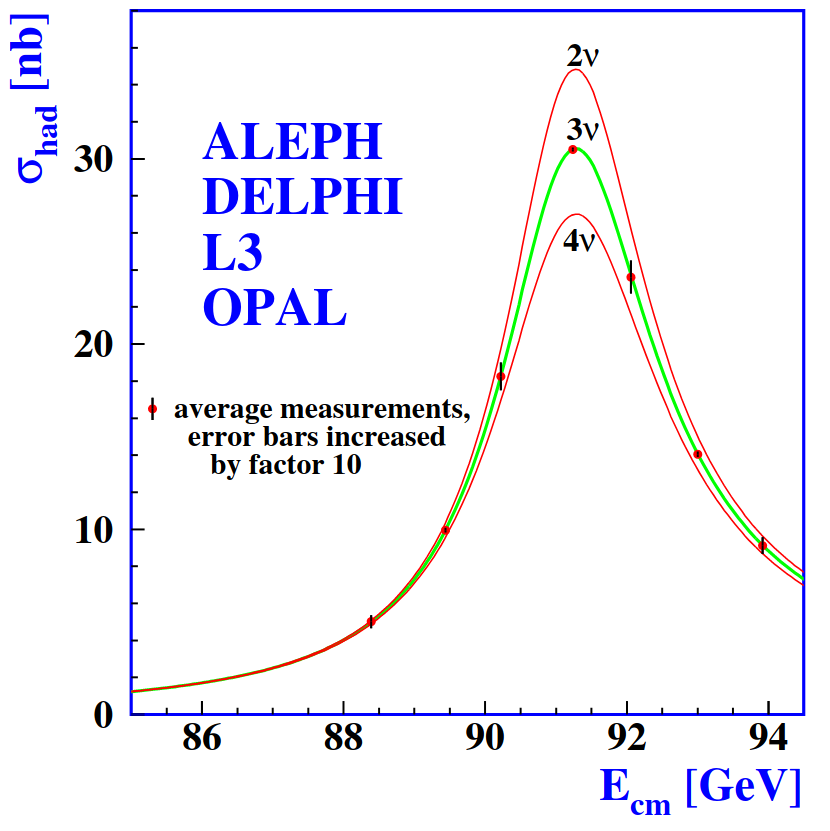
\includegraphics[origin=c,width=0.5\textwidth]{diagrams/3-theory/z_resonance.png}
    \caption[z resonance short]
    {Combined hadron production cross-section measurements around the $Z^{0}$ resonance made by
        experiments at LEP. The curves show the predicted cross-section for two, three, and four
        neutrinos. Note how the data fits the three neutrino hypothesis increadibly well.
        Figure taken from Ref.\cite{electroweak2006}.}
    \label{fig:z_resonance}
\end{figure} %%%%%%%%%%%%%%%%%%%%%%%%%%%%%%%%%%%%%%%%%%%%%%%%%%%%%%%%%%%%%%%%%%%%%%%%%%%%%%%%%%%%%

Combined with the discovery of the tau lepton in 1975~\cite{perl1975}, this suggested that there
was a third tau neutrino. The DONUT experiment at Fermilab finally discovered this particle in
2001~\cite{Kodama2001} using 800\GeV Protons from the Tevatron, completing the trio of neutrinos
we know of today. Any additional neutrinos must either be "sterile"(do not couple to the weak
force) or have a mass greater than $0.5m_{Z}$.

\subsection{Discovery of neutrino oscillations} %%%%%%%%%%%%%%%%%%%%%%%%%%%%%%%%%%%%%%%%%%%%%%%%%%
\label{sec:theory_history_neutrinos}

At the Homestake mine\footnote{The Homestake mine will be used for the future DUNE experiment
    discussed later} in the 1960s, a large tank, placed 1.5 km underground, was filled with
400000 litres of the dry cleaning fluid, perchloroethylene ($C_{4}Cl_{8}$). Its goal was to
measure the solar electron neutrino flux incident upon the earth via the interaction:
\begin{equation} % HOMESTAKE CHLORINE EQUATION %%%%%%%%%%%%%%%%%%%%%%%%%%%%%%%%%%%%%%%%%%%%%%%%%%%
    {}^{37}Cl+\nu_{e}\rightarrow{}^{37}Ar+e^{-},
\end{equation} %%%%%%%%%%%%%%%%%%%%%%%%%%%%%%%%%%%%%%%%%%%%%%%%%%%%%%%%%%%%%%%%%%%%%%%%%%%%%%%%%%%
allowing the neutrino flux to convert the chlorine contained within the tank to the noble gas
argon. Every few weeks the tank was purged with gaseous helium and via a cooled carbon trap the
amount of argon generated, and indirectly the neutrino flux measured.

After analysis, the number of electron neutrino interactions per ${}^{37}Cl$, per second was found
to be no higher than 3~\cite{davis1968}. Compared to the predictions made by the Standard Solar
Model ranging between 4.4 and 22~\cite{bahcall1968}, this indicated a deficit. Dubbed the
'solar neutrino problem', it was initially believed to be due to an unexplained experimental flaw.
However, other experiments, such as the water Cherenkov Kamiokande II~\cite{hirata1989} and both
the SAGE and GALLEX galium based capture tanks also observed this discrepancy.

A neutrino deficit was also observed indirectly in the atmospheric sector. Neutrinos generated in
the atmosphere by cosmic rays formed a key background to the Kamiokande and IMD experiments, both
designed to measure proton decay. When evaluating the background, they observed a deficit in the
number of muon neutrinos compared to electron neutrinos~\cite{hirata1988, becker1992}. The
successor to the Kamiokande experiment Super-Kamiokande also measured the same deficit
~\cite{kajita1999}.

The phenomenon of neutrino oscillations was put forward as a solution to this problem. If
neutrinos could change flavour as they propagated, the measured deficits could be explained. The
SNO experiment finally confirmed this in 2001~\cite{ahmad2002}.

The SNO experiment consisted of a 1 kton tank of deuterium (heavy water), equiped with 9500
photomultiplier tubes. Light from three seperate neutrino interactions channels:
\begin{align} % SNO INTERACTIONS EQUATIONS %%%%%%%%%%%%%%%%%%%%%%%%%%%%%%%%%%%%%%%%%%%%%%%%%%%%%%%
    \nu_{i}+e^{-} & \rightarrow \nu_{i}+e^{-} \\
    \nu_{i}+d     & \rightarrow p+n+\nu_{i}   \\
    \nu_{e}+d     & \rightarrow p+p+e^{-}
\end{align} %%%%%%%%%%%%%%%%%%%%%%%%%%%%%%%%%%%%%%%%%%%%%%%%%%%%%%%%%%%%%%%%%%%%%%%%%%%%%%%%%%%%%%
was measured, where $d$ is the deuterium nucleus. The first and second channels were sensitive to
all three neutrino flavours, but importantly only electron neutrinos could interact via the third
channel. By comparing the rates between the channels, SNO was able to prove to 5.3 sigma that
electron neutrinos had oscillated to other flavours, while the total solar neutrino flux remained
constant.

%%%%%%%%%%%%%%%%%%%%%%%%%%%%%%%%%%%%%%%%%%%%%%%%%%%%%%%%%%%%%%%%%%%%%%%%%%%%%%%%%%%%%%%%%%%%%%%%%%
%                               NEUTRINOS IN THE STANDARD MODEL                                  %
%%%%%%%%%%%%%%%%%%%%%%%%%%%%%%%%%%%%%%%%%%%%%%%%%%%%%%%%%%%%%%%%%%%%%%%%%%%%%%%%%%%%%%%%%%%%%%%%%%
\section{Neutrinos in the Standard Model}
\label{sec:theory_sm}

- The standard model describes all 17 know fundamental particle, six quarks, three charged leptons
three neutrinos, four exchange boson and the higgs boson.
- It unifies the stong force (quantum chromodynamics) with the weak and the electromagnetic forces
(electroweak interactions).
- Neutrinos only interact exclusively via the weak force via W and Z. The weak interaction
maximally violates parity coupling only to left-had-chiral particles, therefore, the SM only
contains left-handed neutrinos (and right-handed antineutrinos).
- Althought not thought of as being in the original standard model, neutrino masses can be
generated, by either including right-handed neutrino fields or including an alternative mass term,
e.g. Majorana mass, or both.
- Regardless of how neutrino masses are generated, it is known that they exist, via infering
from neutrino oscillations which requires them.
- I should then talk about how constraints on the neutrino mass come about.. KATRIN and cosmology
etc...
-
- The standard model is a gauge theory describing the behavoir of all the subatomic particles and
three of the four known forces.
- Lagrangian obeys local gauge symetries described by $U(1) \times SU(2) \times SU(3)$.
- Matter is made of spin 1/2 fermions. This is six quarks and siz leptons, with three generations
of particles, three flavours.
- All particles have an anti-particle with the same quantum numbers, but with an opposite charge
sign.
- Each generation of leptons has a charged lepton and neutral neutrino, e.g. electron and
electron neutrino.
- The charged leptons have the same electric charge and well defined mass, the neutrinos are
neutral and assumed to be massless.
- The quarks carry fractional electric charges, huge range of masses and each carry a "colour"
charge, existing in one of three colours. They never exist in a free state, maybe for a very short
time. And quickly bind to create colourless hadrons.
- Two quarks together is a meson (quark and anti-quark) e.g. pions
- Three quarks together (three quarks of three antiwaurks) is a baryon, e.g. protons, neutrons
- Three forces EM, weak and strong, again hugely different in their relative strengths spanning
many orders of magnitude.
- The forces are carried by spin 1 bosons, EM by photon and affects all charged particles. W and
Z carry the weak force. Strong force whihc binds quarks together over very short-ranges, affects
only colour charged particles and is mediated by the massless gluons (8 of them).
- The higgs is the final elelemtn with gives mass to the particles, via spontaneous symmetry
breaking to W and Z bosons and to fermions via Yukawa couplings.
- Gravity is not incorporated, this is the big problem, but for HEP its not really important as
it significanlty weaker that the ohter forces.
- Neutrinos only interact weakly via W and Z and they are assumed to be massless in the original
SM.
- The original standard model had the neutrinos as massless. But given that neutrinos oscillations
have been observed this is now not valid.
- It is possible to modify the standard model to allow for this fact without new physics, but it
is generally considered to be a significant break in the SM.
- Brief overview of their place in the standard model
- B. Pontecorvo first described neutrino oscillation, by nautrino and anti nuetrinos in 1957,
later Maki, Nakagawa and Sakata in 1962 included electon and muon neutrino mixing
- How does the standard model allow for neutrino masses?
- Fermi vs majorana mass terms, which one is more likely etc
- Free particles travelling in a vacuum can be trated as plane waves $E=\sqrt{p^2+m^2}$ therefore,
the energy eigenstates have a well-defined mass,
this then implies than there must be three mass states for the neutrinos with different quantum
numbers, atleast two must be non-zero.

\begin{figure} % STANDARD MODEL DIAGRAM %%%%%%%%%%%%%%%%%%%%%%%%%%%%%%%%%%%%%%%%%%%%%%%%%%%%%%%%%%
    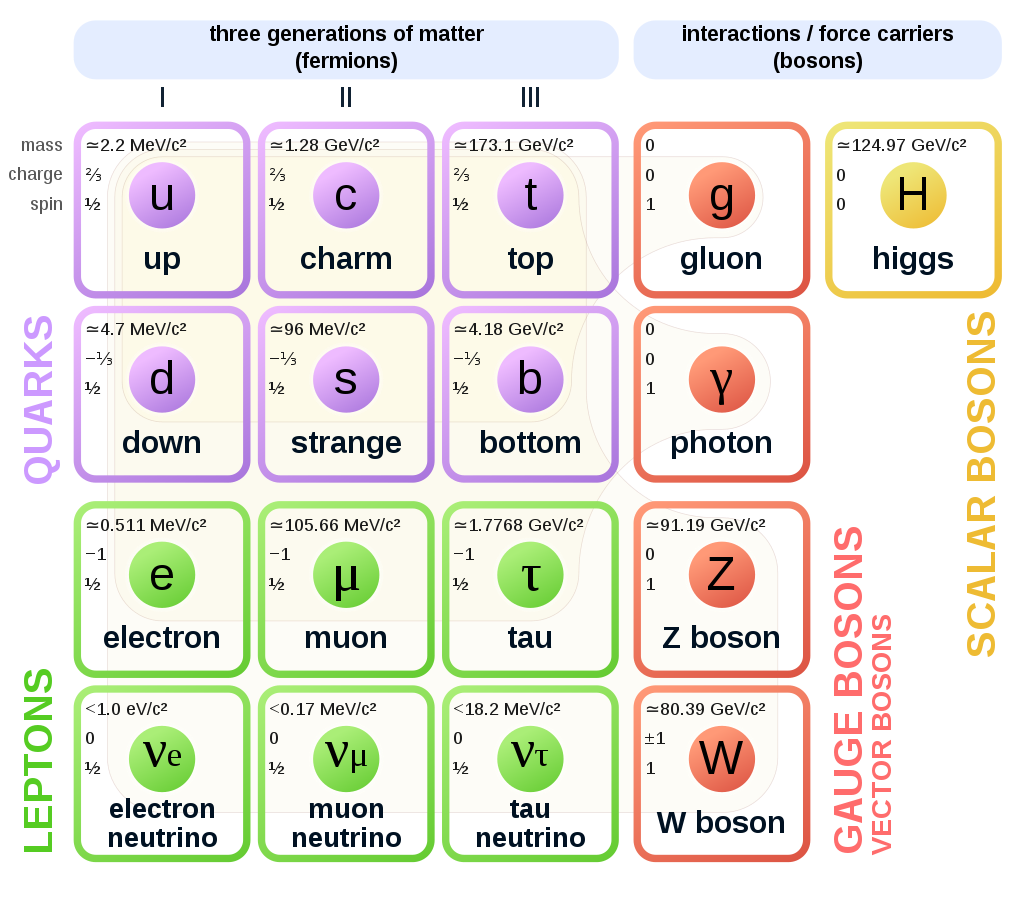
\includegraphics[origin=c,width=0.6\textwidth]{diagrams/3-theory/sm.png}
    \caption[sm short]
    {Figure taken from Ref.\cite{wiki2020}.}
    \label{fig:sm}
\end{figure} %%%%%%%%%%%%%%%%%%%%%%%%%%%%%%%%%%%%%%%%%%%%%%%%%%%%%%%%%%%%%%%%%%%%%%%%%%%%%%%%%%%%%

- Neutrino masses can be Dirac or Majorana. As neutrinos are neutral, they can be their own
anti-particles.
- Best restraints come from cosmological observations of the cosmic microwave background, combined
with other astrophysical data.
-Cosmological mass constraint Ref.~\cite{planck2018} gives $\sum m_{\nu} < 0.12 \eV$ (95\%
confidence level)
- However, these are strongly model-dependent.
- Direct measurements can be made by precise measurements of the beta decay spectrum, as the
maximum energy of  beta decay electron is changed by a non-zero neutrino mass.
-KATRIN Ref.~\cite{aker2019} has measured a model-independent limit just using
kinematics of $m_{\nu} < 1.1 \eV$

%%%%%%%%%%%%%%%%%%%%%%%%%%%%%%%%%%%%%%%%%%%%%%%%%%%%%%%%%%%%%%%%%%%%%%%%%%%%%%%%%%%%%%%%%%%%%%%%%%
%                                NEUTRINO OSCILLATION THEORY                                     %
%%%%%%%%%%%%%%%%%%%%%%%%%%%%%%%%%%%%%%%%%%%%%%%%%%%%%%%%%%%%%%%%%%%%%%%%%%%%%%%%%%%%%%%%%%%%%%%%%%
\section{Neutrino oscillation theory}
\label{sec:theory_oscillations}

\subsection{Neutrino mixing}

The theory of neutrino oscillations was developed in the 1960s by primarily B. Pontecorvo, Z. Maki,
M. Nakagawa, and S. Sakata~\cite{maki1962, pontecorvo1967, pontecorvo1969}.

\begin{equation} % FLAVOUR AS MASS EQUATION %%%%%%%%%%%%%%%%%%%%%%%%%%%%%%%%%%%%%%%%%%%%%%%%%%%%%%%%%
    \ket{\nu_{\alpha}}=\sum_{k}^{3}U_{\alpha k}^{*}\ket{\nu_{k}}
\end{equation} %%%%%%%%%%%%%%%%%%%%%%%%%%%%%%%%%%%%%%%%%%%%%%%%%%%%%%%%%%%%%%%%%%%%%%%%%%%%%%%%%%%%%%

and vice-versa,

\begin{equation} % MASS AS FLAVOUR EQUATION %%%%%%%%%%%%%%%%%%%%%%%%%%%%%%%%%%%%%%%%%%%%%%%%%%%%%%%%%
    \ket{\nu_{k}}=\sum_{\alpha}^{3}U_{\alpha k}\ket{\nu_{\alpha}}
\end{equation} %%%%%%%%%%%%%%%%%%%%%%%%%%%%%%%%%%%%%%%%%%%%%%%%%%%%%%%%%%%%%%%%%%%%%%%%%%%%%%%%%%%%%%


where $\alpha = e, \mu, \tau$

- The theory of neutrino oscillation was developed by Pontecorvo, Maki, Nakagawa, and Sakata.
- Neutrino mixing desribes the superposition of neutrino mass eigenstates within neutrino flavour
eigenstates.
- U in the Pontecorvo-Maki-Nakagawa-Sakara (PMNS) matrix.
- The basic forms assumes neutrinos are Dirac in nature and not their own anti-particle. if
neutrinos are Majorana particles, two additional CPV phases need to be added to the matrix to
fully describe the mixing.
- Oscillations arise because the three weak interactin eigenstates are not that same as the three
mass eigenstates, but are formed from a linear combination as defined by the PMNS matrix.
- The changing state of the neutrino flavour as it propogates can be explained by having the
flavour eigenstates through which the neutrinos
couple to the weak force be different from their energy eigenstates for the matter through which
the neutrinos are travelling.
- With the flavour eigenstates being expresses as a superposition of the energy states, neutrino
oscillations arise through interference due tof
the energy states evolving differently with time.
- Can be explained by the quantum pheneomentum of interferance.
- With the flavour and mass eigenstates not being evuivalent, this mixing is described by the
rotation PMNS matrix, analogous to the CKM mixing describing mixing in the quark sector.
- To understand neutrinos you need, a flavour basis, an orthonormal energy basis with three energy
esigenstates for the medium, eigenvalues of those energy states,
and a unitary matrix to convert between the basis.
- In a vacuum, a unitary mixing matrix describes the mixing of mass states to produce the flavour
states. and vice-versa
- In the case of three neutrino flavours the unitary mixing matrix is called the Pontecorvo, Maki,
Nakata and Sakawa matrix, PMNS.
- Analagous to the CKM (Cabibbo-Kobayashi-Maskawa) matrix.
- $\mathrm{U}_{\mathrm{PMNS}}$ is a unitary, complex, $3\times3$ matrix. Which can be desribed by
$n^{2}$ parameters, with $n(n-1)/2$ angles
and $n(n+1)/2$ phases, 3 mixing angles $\theta_{12}$, $\theta_{23}$ and $\theta_{13}$ and six
complex phases.
- Some of these phases can be removed as it desribes the mixing between particle fields, hence no
physical processes are affected.
- They are absorbed into the neutrino fields.
- If Dirac particles then just one pahse is left $\delta_{CP}$ if Majorana you get an additional
two phases $\alpha_{12}$ and $\alpha_{31}$ which lie on the diagonal and hence have no effect on
neutrino oscillations.

\begin{gather} % PMNS MATRIX SIMPLE %%%%%%%%%%%%%%%%%%%%%%%%%%%%%%%%%%%%%%%%%%%%%%%%%%%%%%%%%%%%%%
    \begin{pmatrix}
        \ket{\nu_{e}}   \\
        \ket{\nu_{\mu}} \\
        \ket{\nu_{\tau}}
    \end{pmatrix}
    =
    \begin{pmatrix}
        U_{e1}     & U_{e2}     & U_{e3}     \\
        U_{\mu 1}  & U_{\mu 2}  & U_{\mu 3}  \\
        U_{\tau 1} & U_{\tau 2} & U_{\tau 3}
    \end{pmatrix}
    \begin{pmatrix}
        \ket{\nu_{1}} \\
        \ket{\nu_{2}} \\
        \ket{\nu_{3}}
    \end{pmatrix}
\end{gather} %%%%%%%%%%%%%%%%%%%%%%%%%%%%%%%%%%%%%%%%%%%%%%%%%%%%%%%%%%%%%%%%%%%%%%%%%%%%%%%%%%%%%

\begin{align} % DIRAC PMNS MATRIX FULL %%%%%%%%%%%%%%%%%%%%%%%%%%%%%%%%%%%%%%%%%%%%%%%%%%%%%%%%%%%
    \mathrm{U}_{\mathrm{PMNS}} & =
    \begin{pmatrix}
        1 & 0       & 0      \\
        0 & c_{23}  & s_{23} \\
        0 & -s_{23} & c_{23}
    \end{pmatrix}
    \begin{pmatrix}
        c_{13}                   & 0 & s_{13}e^{-i\delta_{CP}} \\
        0                        & 1 & 0                       \\
        -s_{13}e^{-i\delta_{CP}} & 0 & c_{13}
    \end{pmatrix}
    \begin{pmatrix}
        c_{12}  & s_{12} & 0 \\
        -s_{12} & c_{12} & 0 \\
        0       & 0      & 1
    \end{pmatrix}
    \\
                               & =
    \begin{pmatrix}
        c_{12}c_{13}
         & s_{12}c_{13}
         & s_{13}e^{-i\delta_{CP}}                          \\
        -s_{12}c_{23}-c_{12}s_{23}s_{13}e^{i\delta_{CP}}
         & c_{12}c_{23}-s_{12}s_{23}s_{13}e^{i\delta_{CP}}
         & s_{23}c_{13}                                     \\
        s_{12}s_{23}-c_{12}c_{23}s_{13}e^{i\delta_{CP}}
         & -c_{12}s_{23}-s_{12}c_{23}s_{13}e^{i\delta_{CP}}
         & c_{23}c_{13}
    \end{pmatrix}
\end{align} %%%%%%%%%%%%%%%%%%%%%%%%%%%%%%%%%%%%%%%%%%%%%%%%%%%%%%%%%%%%%%%%%%%%%%%%%%%%%%%%%%%%%%

with $s_{ij}=\sin \theta_{ij}$ and $c_{ij}=\cos \theta_{ij}$

\begin{align} % MAJORANA DIAGONAL PMNS EQUATION %%%%%%%%%%%%%%%%%%%%%%%%%%%%%%%%%%%%%%%%%%%%%%%%%%
    M = \mathrm{diag}(1, e^{i\phi_{1}}, e^{i\phi_{2}})
\end{align} %%%%%%%%%%%%%%%%%%%%%%%%%%%%%%%%%%%%%%%%%%%%%%%%%%%%%%%%%%%%%%%%%%%%%%%%%%%%%%%%%%%%%%

\subsection{Oscillations in vacuum}

To calculate the oscillation probabilities for neutrinos produced in a given flavourstate, we must
use the mixing matrix to convert into the basis of energy eigenstates,evolve these in time, and
project the evolved states back into the flavour basis usingthe mixing matrix once more.  This
yields an amplitude which can then be squaredto produce the oscillation probability.

The neutrino mass states are eigenstates of the hamiltonian with energy eigenvalues $E_{k}$:
\begin{equation} % HAMILTONIAN EQUATION %%%%%%%%%%%%%%%%%%%%%%%%%%%%%%%%%%%%%%%%%%%%%%%%%%%%%%%%%%
    H \ket{\nu_{k}} = E_{k} \ket{\nu_{k}}.
    \label{eq:hamiltonian}
\end{equation} %%%%%%%%%%%%%%%%%%%%%%%%%%%%%%%%%%%%%%%%%%%%%%%%%%%%%%%%%%%%%%%%%%%%%%%%%%%%%%%%%%%
This allows the time evolution of the flavour eigenstates to be written using the
Schr$\mathrm{\ddot{o}}$dinger equation, such that,
\begin{equation} % TIME EVOLUTION EQUATION %%%%%%%%%%%%%%%%%%%%%%%%%%%%%%%%%%%%%%%%%%%%%%%%%%%%%%%
    \ket{\nu_{\alpha}(t)}=\sum_{k}^{3}U_{\alpha k}^{*}e^{-iE_{k}t}\ket{\nu_{k}}.
    \label{eq:time_evolution_1}
\end{equation} %%%%%%%%%%%%%%%%%%%%%%%%%%%%%%%%%%%%%%%%%%%%%%%%%%%%%%%%%%%%%%%%%%%%%%%%%%%%%%%%%%%
The oscillation probability is thus equal to,
\begin{equation} % TIME EVOLUTION EQUATION %%%%%%%%%%%%%%%%%%%%%%%%%%%%%%%%%%%%%%%%%%%%%%%%%%%%%%%
    P(\nu_{\alpha} \rightarrow \nu_{\beta}, t) = |\braket{\nu_{\beta}|\nu_{\alpha}(t)}|^{2}=
    \abs*{\sum_{k}^{3}U_{\alpha k}^{*}U_{\beta k}e^{-iE_{k}t}}^{2} \\
    =\sum_{k}^{3}\sum_{j}^{3}U_{\alpha k}^{*}U_{\beta k}U_{\alpha j}U_{\beta j}^{*}
    e^{i(E_{k}-E_{j})t}.
    \label{eq:osc_prob}
\end{equation} %%%%%%%%%%%%%%%%%%%%%%%%%%%%%%%%%%%%%%%%%%%%%%%%%%%%%%%%%%%%%%%%%%%%%%%%%%%%%%%%%%%
As neutrinos are ultrarelativistic ($p\simeq E$) the approximation,
\begin{equation} % ENERGY, MASS, MOMENTUM EQUATION %%%%%%%%%%%%%%%%%%%%%%%%%%%%%%%%%%%%%%%%%%%%%%%
    E_{k}=\sqrt{\vec{p}_{k}^{\,2}+m_{k}^{2}}\simeq E+\frac{m_{k}^{2}}{2E},
    \label{eq:energy_mass_momentum}
\end{equation} %%%%%%%%%%%%%%%%%%%%%%%%%%%%%%%%%%%%%%%%%%%%%%%%%%%%%%%%%%%%%%%%%%%%%%%%%%%%%%%%%%%
where E is the neutrino energy without the mass, can be used to give,
\begin{equation} % ENERGY, MASS, MOMENTUM EQUATION %%%%%%%%%%%%%%%%%%%%%%%%%%%%%%%%%%%%%%%%%%%%%%%
    E_{k}-E_{j}\approx\frac{\Delta m_{kj}^{2}}{2E}
    \label{eq:energy_mass_momentum}
\end{equation} %%%%%%%%%%%%%%%%%%%%%%%%%%%%%%%%%%%%%%%%%%%%%%%%%%%%%%%%%%%%%%%%%%%%%%%%%%%%%%%%%%%
where $\Delta m_{kj}^{2}$ is the squared mass difference (mass splitting) between the $i$th and
$j$th mass states. Combined with taking $t = L$ again due to the ultrarelativistic limit, and some
trigonometric identities,
\begin{align} % TIME EVOLUTION EQUATION %%%%%%%%%%%%%%%%%%%%%%%%%%%%%%%%%%%%%%%%%%%%%%%%%%%%%%%
    P(\nu_{\alpha} \rightarrow \nu_{\beta}, t) = \delta_{\alpha\beta} & - 4\sum_{k>j}re(
    U_{\alpha k}^{*}U_{\beta k}U_{\alpha j}U_{\beta j}^{*})\sin^{2}\left(\frac{\Delta
        m_{kj}^{2}L}{4E}\right)
    \\  & \pm 2\sum_{k>j}im(
    U_{\alpha k}^{*}U_{\beta k}U_{\alpha j}U_{\beta j}^{*})\sin\left(\frac{\Delta
        m_{kj}^{2}L}{4E}\right).
    \label{eq:osc_prob}
\end{align} %%%%%%%%%%%%%%%%%%%%%%%%%%%%%%%%%%%%%%%%%%%%%%%%%%%%%%%%%%%%%%%%%%%%%%%%%%%%%%%%%%%

- Oscillations are driven by the mass-squared differences between the mass eignestates.
- Talk about the full neutrino oscillation equations, but also the simplified ones and then how
they affect the shape of the probability curves.
INFO: How the shape of the neutrino flux at the far detector affects the parameters, reduction
fraction, position of the dip etc... maybe a little diagram
- Using the simplified approximation of treating the neutrino states as plane waves, we can simply
derive the oscilaltion probabilities.
- Main flaw with this assumption is that plane waves are not localised and can not describe the
localised interactions of neutrinos.
- Additionally neutrinos have differing energy and momentum not a common one approximation as c.
- These can be solved when the neutrino states are described as wave packets, but this derivation
is much simpler and gets to the same equally correct result.
- The energy state propogation is well defined, causing the neutrino flavour to change with time
in an oscillatory fashion. Such that a muon neutrino after travelling a distance can be detected
as a electon of tau neutrino but after another distance be detector as a muon neutrino again.

\subsection{Oscillations in matter}

Wolfenstein oscillations in matter paper Ref.~\cite{wolfenstein1978}
Mikheyev oscillations in matter paper Ref.~\cite{mikheev1986}
Numu to nuel oscilaltion probability equation Ref.~\cite{cervera2000}

\begin{figure} % OSCILLATION MATTER PROBS DIAGRAM %%%%%%%%%%%%%%%%%%%%%%%%%%%%%%%%%%%%%%%%%%%%%%%%
    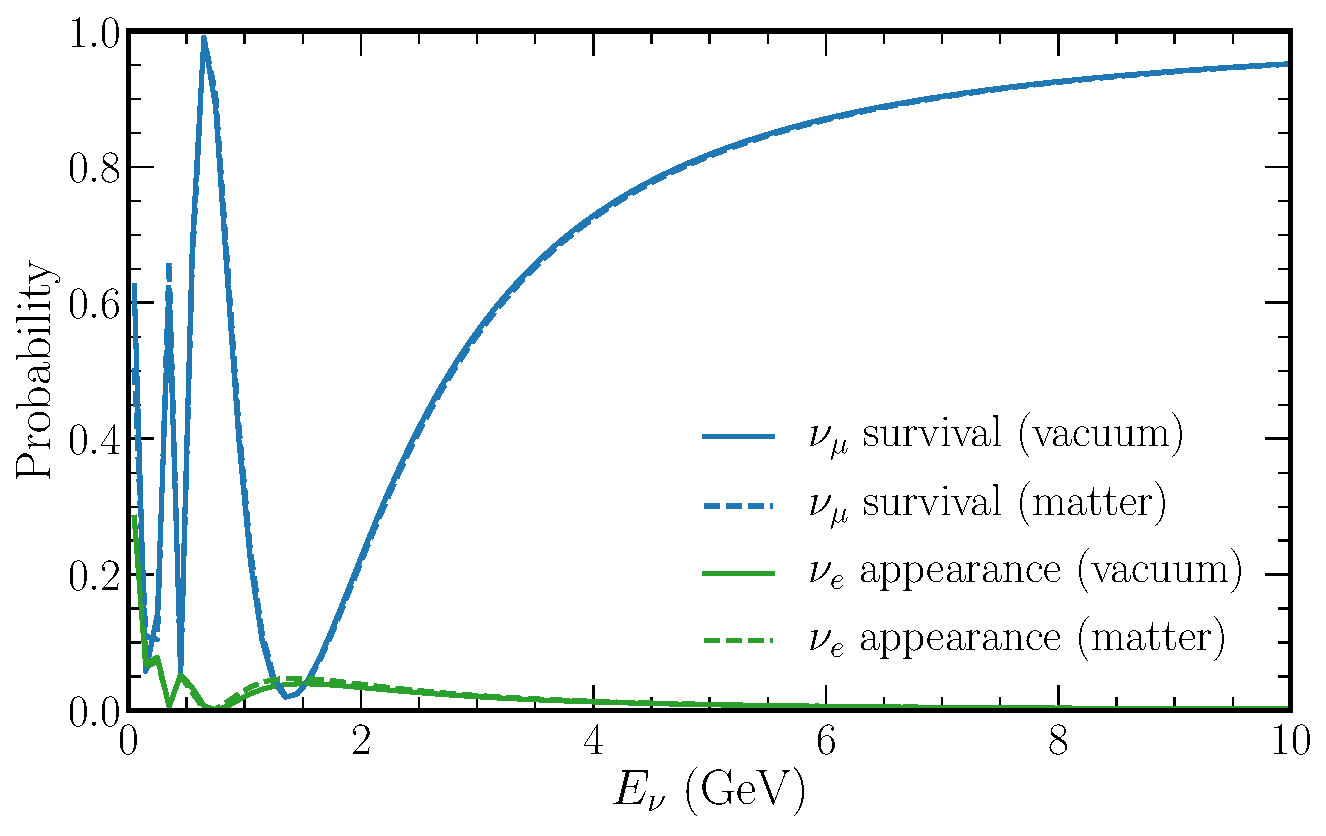
\includegraphics[origin=c,width=0.8\textwidth]
    {diagrams/3-theory/explore_osc_vac_vs_matter_probs.pdf}
    \caption[osc matter probs short]
    {osc matter probs long}
    \label{fig:osc_matter_probs}
\end{figure} %%%%%%%%%%%%%%%%%%%%%%%%%%%%%%%%%%%%%%%%%%%%%%%%%%%%%%%%%%%%%%%%%%%%%%%%%%%%%%%%%%%%%

\begin{figure} % OSCILLATION CP PROBS DIAGRAM %%%%%%%%%%%%%%%%%%%%%%%%%%%%%%%%%%%%%%%%%%%%%%%%%%%%
    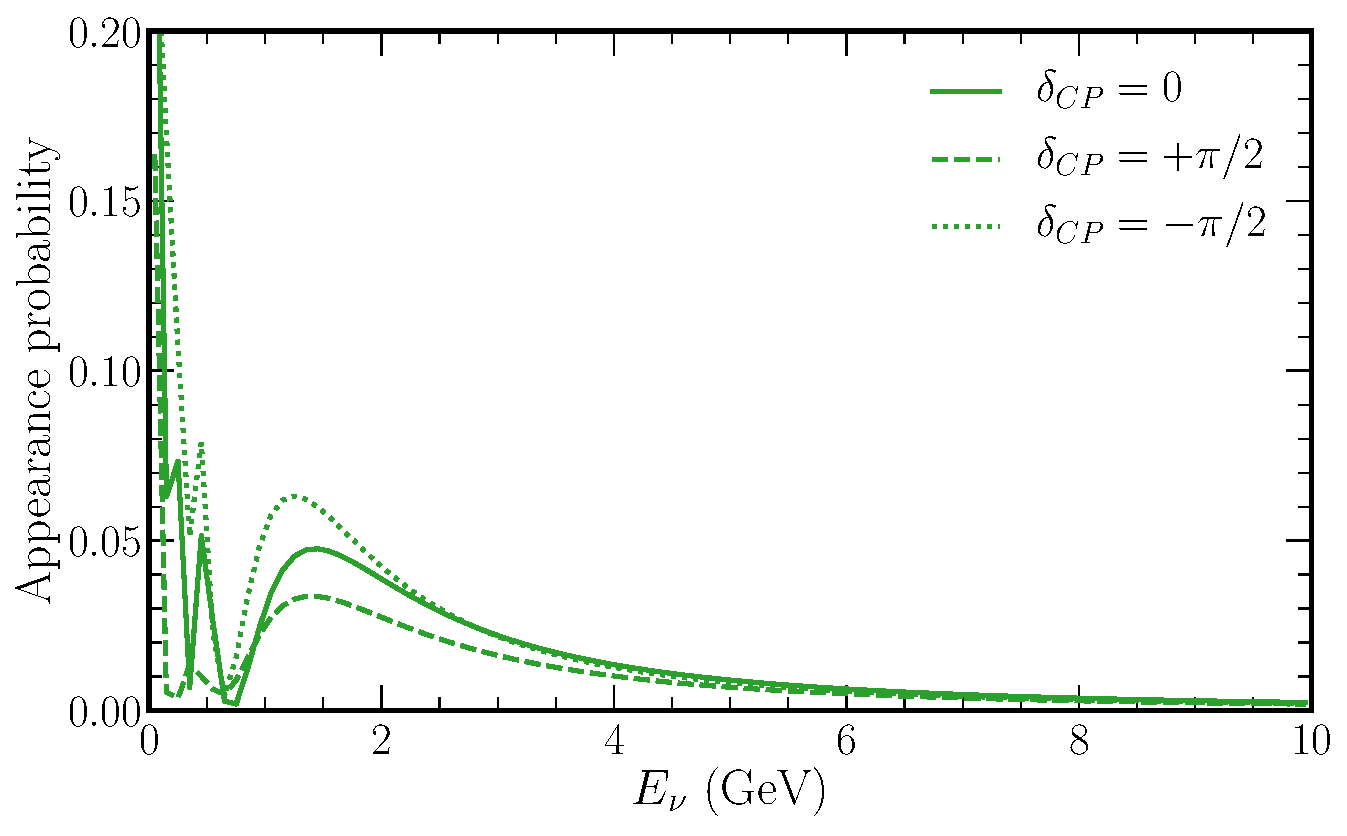
\includegraphics[origin=c,width=0.8\textwidth]{diagrams/3-theory/explore_osc_cp_probs.pdf}
    \caption[osc cp probs short]
    {osc cp probs long}
    \label{fig:osc_cp_probs}
\end{figure} %%%%%%%%%%%%%%%%%%%%%%%%%%%%%%%%%%%%%%%%%%%%%%%%%%%%%%%%%%%%%%%%%%%%%%%%%%%%%%%%%%%%%

%%%%%%%%%%%%%%%%%%%%%%%%%%%%%%%%%%%%%%%%%%%%%%%%%%%%%%%%%%%%%%%%%%%%%%%%%%%%%%%%%%%%%%%%%%%%%%%%%%
%                                 CURRENT STATUS AND THE FUTURE                                  %
%%%%%%%%%%%%%%%%%%%%%%%%%%%%%%%%%%%%%%%%%%%%%%%%%%%%%%%%%%%%%%%%%%%%%%%%%%%%%%%%%%%%%%%%%%%%%%%%%%
\section{Current status and the future}
\label{sec:theory_status}

\subsection{Current experimental status}

Daya bay theta13 Ref.~\cite{an2012}
RENO theta13 Ref.~\cite{ahn2012}
Double Chooz theta13 Ref.~\cite{abe2012}

\subsection{Open question}

\begin{figure} % MASS HIERARCHY DIAGRAM %%%%%%%%%%%%%%%%%%%%%%%%%%%%%%%%%%%%%%%%%%%%%%%%%%%%%%%%%%
    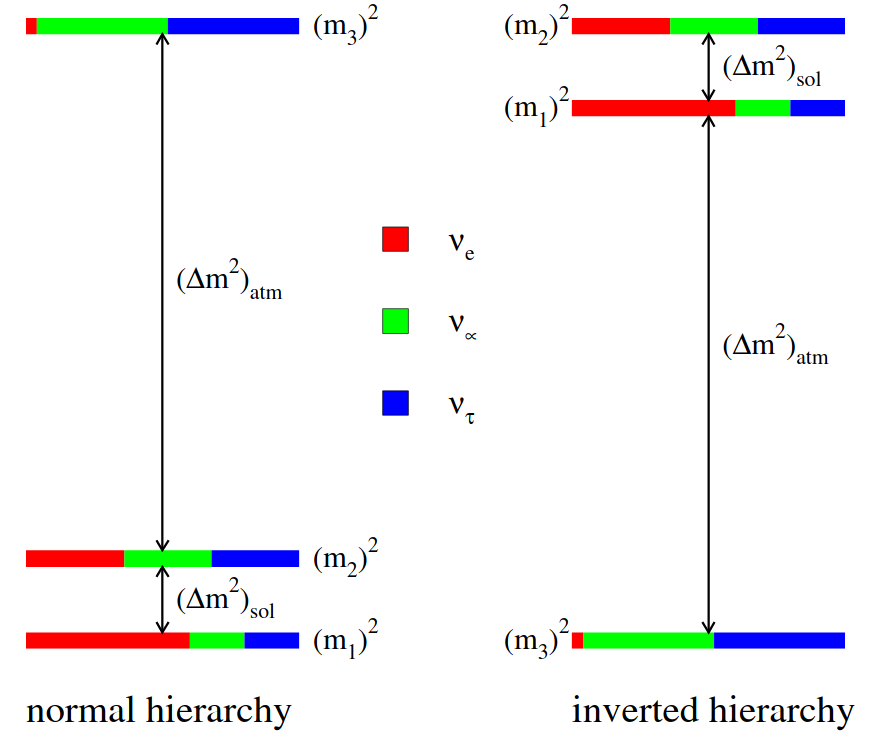
\includegraphics[origin=c,width=0.6\textwidth]{diagrams/3-theory/hierarchy.png}
    \caption[hierarchy short]
    {Figure taken from Ref.\cite{gouvea2013}.}
    \label{fig:hierarchy}
\end{figure} %%%%%%%%%%%%%%%%%%%%%%%%%%%%%%%%%%%%%%%%%%%%%%%%%%%%%%%%%%%%%%%%%%%%%%%%%%%%%%%%%%%%%


\subsection{Future experiments}

\begin{comment}
- With the measurements of a non-zero theta13 by reactor neutrino experiments, the main focus now
has shifted to resolving the mass hierarchy ambiguity and measuring delta-cp. These can be probed
by long-baseline neutrino experiments by looking to numu to nuel transitions.
- BIG EQUATION FOR PROBABILITY: shows sensitivity to the mass hiearchy through the matter effect
parameters A and to the cp-violtating phase trhough the second term.
- Over that last 20 years neutrino oscillations have become well-established and we are now moving
into the precision measurement era.
- DUNE is a next-generation neutrino oscillation experiment with a primary scientific goal of
observation of CP-violation in the neutrino sector.
- In DUNE a muon neutrino(anti-neutrino) beam will be produced by the Long-Baseline Neutrino
Facility (LBNF)
- There will be a near detector at Fermilab before the neutrinos travel the 1285km to the Sanford
Underground Research Facility (SURF) in South Dakota.
- The far detector will consist of four 10kt (fiducial) liquid argon time projections chamber
(LArTPC) detectors.
- Neutrino oscillation probabilities can then be infered by comparisons of the observed neutrino
spectra and the near and far detectors.
- Recent obsevation of a large theta13 have focuseed the next genetation of long baseline
experiments towards the mass hierarchy, octant of theta23 and measureing delta-CP
- Nova and T2k will not be able to measure the remaining unknows (check this)
- Dune will hopefully solve these problems but will be increadibly expensive

- Symmetries under charge-conjugation and parity inversion are both macimally violated by the
waek interaction.
- Their combined operation has been shown to be violated, to a small degress, by quark mixing
processes.
- If sin(delta-cp) is non zero then vacuum oscillation properties of nu and anti nu will be
different.
- DUNE (I assume CHIPS) is sensative to four oscillation paramters, delta31, theta23, theta13
and delta-cp.
- These can be measured using four data sample, two for neutrino and two for antineutrinos.
- These sample are produced by "Forward Horn current" FHC and "Reverse Horn current" RHC,
producing predominetetly neutrinos and anti-neutrinos respectively.
- Dissapearence channels sensitive to %abs(delta31^2), and sin^2(2theta23).
- Apperence channels sensitive to all four parameters including sign of %delta32^2.
- The "signal" in all cases are CC interactions, therefore selection of nuel, anuel, numu and
anumu CC is the goal.
- Main background in CC numu selections are NC with charged pions.
- Main background in CC nuel selections is pi-zero NC, which can mimic the chracteristic EM
shower, due to its near certain decay into two photons.
- You get a small number of nuel intrinsic to the beam, they are just a background as they are
indistinguishabe from the nuel appreaence neutrinos.
- Once you have collected samples in all four cases, a fit is performed to the reconstructed
neutrino energy distributions to extract the four neutrino oscillation parameters.
- How is the absolute nuetrino energy constrained\dots
- KATRIN upper limit of 1.1eV (90percent confidence level) on the absolute mass of the neutrinos.
KATRIN mass in in Ref.~\cite{aker2019}
\end{comment}